\subsection{Kernel Density Estimation}
\label{sub:kernelDensityEstimation}

Finding a local crowd density can be a simple task. Simply define the local area, and count the number of people inside that areas, and divide it by the size of the local area. This process could then be repeated across multiple local areas, to give us the the local densities across the entire area. These counts could then be displayed in histograms for a better overview. The problem with this approach is the definition of the local areas. Whatever way you decide to define the areas will affect the outcome of the count, which in turn will affect the histograms, giving a possibly skewed overview\kanote{jens, insert article reference here}. Since we do not want this, we need to use a different method.

%--- Jens' formulering --- %
%To calculate the local crowd density, one could place a grid over the area, count the number of people in each square and divide by the area of the square. This can be done with histograms. The problem with this method is its sensitivity to the grid, and that inaccuracies in the measured positions are not accounted for.\jenote{Complete the argumentation for why we should use kernel density estimation rather than histograms}

\kanote{mangler en overgang fra problemet med histogrammer til kernel density estimation}

There exists multiple kernel functions that can be used in the kernel density estimation. The most commonly used is the Gaussian distribution, also known as the normal distribution, given by the function in \cref{eq:1dGaussianDistribution}. The function, given the distance $d$ from an observation to the center of the kernel, returns the probability of the observation. An observation in this context, is a sample drawn from the distribution. The Gaussian distribution is commonly used as a kernel function because it arises naturally, both in theory and in experiments.

\begin{equation}
\label{eq:1dGaussianDistribution}
K(d) = \frac{1}{\sqrt{2\pi}} e^{-\frac{1}{2} d^2}
\end{equation}

The plot of the function is shown in \cref{fig:1dGaussianDistributionPlot}. Notice that the function only converges with the x axis in $-\infty$ and $\infty$. This means that if we were to use this function for calculating the local crowd density, we would have to consider every person in the data set, because the function is defined for every x value. For performance reasons, this is not preferable.

Another kernel function is the Epanechnikov kernel, given by the function in \cref{eq:1dEpanechnikovDistribution}.

\begin{equation}
\label{eq:1dEpanechnikovDistribution}
K(d) = \frac{3}{4} \left( 1-d^2 \right) \mathbbm{1}_{\{\left| d \right| \leq 1\}}
\end{equation}

Here $\mathbbm{1}_{\{|d| \leq 1\}}$ denotes the indicator function, meaning that if $|d|$ has a value less than or equal to 1, the function returns $0$, otherwise $1$. This means that any person placed outside this range in our data set can be ignored. This property can be seen in the plot of the function in \cref{fig:1dEpanechnikovDistributionPlot}, where one can also see that the function converges with the x axis at $-1$ and $1$.
\lanote{Maybe remove this graph and use the one with the area marked instead}

\begin{figure}[htbp]
\begin{subfigure}[c]{.49\linewidth}
    \centering
    \begin{tikzpicture}[scale=0.9]
    \begin{axis}[
    axis y line=center,
    axis x line=middle,
    grid=both,
    xmin=-3,xmax=3,
    ymin=-0.2,ymax=1,
    xlabel=$x$,ylabel=$y$,
    x label style={at={(axis description cs:1,0.2)},anchor=east},
    y label style={at={(axis description cs:0.5,1)},anchor=north west},
    xtick={-3,-2,-1,0,1,2,3},
    ytick={-0.2,0,0.1,0.2,0.3,0.4,0.5,0.6,0.7,0.8,0.9,1},
    height=7.5cm,
    anchor=center]
    \addplot[mark=none, thick, samples=100, smooth, domain=-1:1] {epanechnikov2d(1)};
    \addplot[mark=none, thick, samples=100, smooth, domain=1:3] {0};
    \addplot[mark=none, thick, samples=100, smooth, domain=-1:-3] {0};
    \end{axis}
    \end{tikzpicture}
    \caption{Epanechnikov distribution}
    \label{fig:1dEpanechnikovDistributionPlot}
\end{subfigure}
%
\begin{subfigure}[c]{.49\linewidth}
    \centering
    \begin{tikzpicture}[scale=0.9]
    \begin{axis}[
    axis y line=center,
    axis x line=middle,
    grid=both,
    xmin=-3,xmax=3,
    ymin=-0.2,ymax=1,
    xlabel=$x$,ylabel=$y$,
    x label style={at={(axis description cs:1,0.2)},anchor=east},
    y label style={at={(axis description cs:0.5,1)},anchor=north west},
    xtick={-3,-2,-1,0,1,2,3},
    ytick={-0.2,0,0.1,0.2,0.3,0.4,0.5,0.6,0.7,0.8,0.9,1},
    height=7.5cm,
    anchor=center]
    \addplot[mark=none, thick, samples=100, smooth] {gaussian2d(1)};
    \end{axis}
    \end{tikzpicture}
    \caption{Gaussion/normal distribution}
    \label{fig:1dGaussianDistributionPlot}
\end{subfigure}
\caption{Kernel density function plots}
\end{figure}

Choosing a kernel function is not very important as long as the chosen function has an area of 1 beneath it.\jenote{find source} The area of both functions can be seen plotted in \cref{fig:1dGaussianEpanechnikovAreaPlot}. While both Gaussian and Epanechnikov hold this property, Epanechnikov was chosen because it is not defined for every x value, making its performance advantageous. There are many other kernel functions that also apply the indicator function and has an area of 1 beneath its curve which could have been considered. However since the choice of the kernel function is of minor importance, we did not pursue other options.

\begin{figure}[htbp]
\begin{subfigure}[c]{.49\linewidth}
    \centering
    \begin{tikzpicture}[scale=0.9]
    \begin{axis}[
    axis y line=center,
    axis x line=middle,
    grid=both,
    xmin=-3,xmax=3,
    ymin=-0.2,ymax=1,
    xlabel=$x$,ylabel=$y$,
    x label style={at={(axis description cs:1,0.2)},anchor=east},
    y label style={at={(axis description cs:0.5,1)},anchor=north west},
    xtick={-3,-2,-1,0,1,2,3},
    ytick={-0.2,0,0.1,0.2,0.3,0.4,0.5,0.6,0.7,0.8,0.9,1},
    height=7.5cm,
    anchor=center]
    \addplot[mark=none, thick, samples=100, smooth, domain=-1:1] {epanechnikov2d(1)};
    \addplot[mark=none, thick, samples=100, smooth, domain=1:3] {0};
    \addplot[mark=none, thick, samples=100, smooth, domain=-1:-3] {0};
    \addplot[mark=none, thick, samples=100, smooth, fill=lightgray, fill opacity=0.5, domain=-1:1] {epanechnikov2d(1)};
    \end{axis}
    \end{tikzpicture}
    \caption{Epanechnikov distribution}
    \label{fig:1dEpanechnikovAreaPlot}
\end{subfigure}
%
\begin{subfigure}[c]{.49\linewidth}
    \centering
    \begin{tikzpicture}[scale=0.9]
    \begin{axis}[
    axis y line=center,
    axis x line=middle,
    grid=both,
    xmin=-3,xmax=3,
    ymin=-0.2,ymax=1,
    xlabel=$x$,ylabel=$y$,
    x label style={at={(axis description cs:1,0.2)},anchor=east},
    y label style={at={(axis description cs:0.5,1)},anchor=north west},
    xtick={-3,-2,-1,0,1,2,3},
    ytick={-0.2,0,0.1,0.2,0.3,0.4,0.5,0.6,0.7,0.8,0.9,1},
    height=7.5cm,
    anchor=center]
    \addplot[mark=none, thick, samples=100, smooth] {gaussian2d(1)};
    \addplot[mark=none, thick, samples=100, smooth, fill=lightgray, fill opacity=0.5, restrict y to domain=0:1] {gaussian2d(1)};
    \end{axis}
    \end{tikzpicture}
    \caption{Gaussian/normal distribution}
    \label{fig:1dGaussianAreaPlot}
\end{subfigure}
\caption{The area beneath both Epanechnikov and the Gaussian distribution}
\label{fig:1dGaussianEpanechnikovAreaPlot}
\end{figure}

A kernel density estimation is performed for a specific point, and can be calculated as either absolute, relative, or probabilistic density. The absolute density is the amount of people per local crowd density point. This means that the densities for all points have to sum up to the total amount of people.

The relative densities are the absolute densities divided by the area that each point covers, for instance people per square meter. Since we want to be able to compare the values calculated for the crowd factors with certain limits, this is the type of kernel density we want to calculate.

The last kernel density type is probabilistic. This is the absolute densities divided by the total amount of people, meaning that the total sum of probabilistic local crowd densities has to be 1.

Kernel functions have an area of 1 beneath them since they denote the probability of finding an observation at certain distances from them. In essence this means that all observations exist in the distribution of the function. In our case, this denotes how much a observed person weighs for the density of the point. The problem is that observations can exist further away than a distance of 1. We assume that all distances are in SI unit meters. We want a way to raise or lower the distance of observations that should be considered in the estimation, in order to include all observations of importance, but still have the kernel density functions have an area of 1. This is done using a bandwidth variable. The Epanechnikov function with the bandwidth can be seen in \cref{eq:1dEpanechnikovDistributionWithH} and the plot of the function is shown in \cref{fig:1dEpanechnikovDistributionWithHPlot} with the area underneath. The area of this function is still 1 and therefore holds the property of a kernel density function.

\begin{equation}
\label{eq:1dEpanechnikovDistributionWithH}
K(d) = \frac{3}{4 h} \left( 1-\left(\frac{d}{h}\right)^2 \right) \mathbbm{1}_{\{|u| \leq 1\}}
\end{equation}

Here $d$ is the distance from the center of the kernel function to the observation, and $h$ is the bandwidth.

\begin{figure}
\centering
\begin{tikzpicture}[baseline]
\begin{axis}[
axis y line=center,
axis x line=middle,
grid=both,
xmin=-6,xmax=6,
ymin=-0.2,ymax=1,
xlabel=$x$,ylabel=$y$,
x label style={at={(axis description cs:1,0.2)},anchor=east},
y label style={at={(axis description cs:0.5,1)},anchor=north west},
xtick={-5,...,5},
ytick={-0.2,-0.1,0,0.1,0.2,0.3,0.4,0.5,0.6,0.7,0.8,0.9,1},
width=10cm,
height=7.5cm,
anchor=center]
\addplot[mark=none, thick, samples=100, smooth, domain=-6:-5] {0};
\addplot[mark=none, thick, samples=100, smooth, domain=5:6] {0};
\addplot[mark=none, thick, samples=100, smooth, fill=lightgray, fill opacity=0.5, domain=-5:5] {epanechnikov2d(5)};
\end{axis}
\end{tikzpicture}
\caption{The area beneath the Epanechnikov function with bandwidth 5}
\label{fig:1dEpanechnikovDistributionWithHPlot}
\end{figure}

Currently we have only been looking at the distribution over one dimension. In our domain we get observations from a plane, in two dimensions. We can extend the kernel function to work on a two dimensional area by calculating the distance from the kernel function center point to the desired point in two dimensions. In 2 dimensions, the distance would be the same as a radius in a circle. This can be seen plotted in \cref{fig:3dEpanechnikov}.

\begin{figure}[htbp]
\centering
    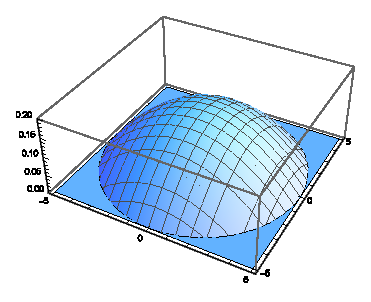
\includegraphics[width=0.5\textwidth]{3dEpanechnikov.eps}
    \caption{Epanechnikov over an area shown in 3 dimensions.}
    \label{fig:3dEpanechnikov}
\end{figure}

\Cref{fig:3dEpanechnikov} represents the distribution over a 2 dimensional space, where the third dimension represents how much the 2 dimensional points weights.

As explained earlier, the function is currently on a probability form, and not on the desired relative density form. In order to modify it, we first transform it to an absolute form. People closer to a point will weigh more than people further away from the point. We assume that every person contributes the same density, so the mean value of the function should be 1. In order to \enquote{raise} the function so the mean value is 1, we can divide by the volume beneath the plane and multiply with the desired volume. The desired volume is that of which the kernel function has a mean value of 1. We start by calculating the current volume beneath the plane. This can be done through a triple integration on the function using a circular coordinate set. As defined previously, the distance from point to center is the radius. The integration is done as shown in \cref{eq:volumeUnder3dEpanechnikov}.

\begin{equation}
\label{eq:volumeUnder3dEpanechnikov}
\int_0^{2 \pi} \int_0^h \int_0^1 \frac{3}{4 h} \left(1 - \left(\frac{r}{h}\right)^2\right) \mathrm{d}z\ \mathrm{d}r\ \mathrm{d}\theta\ = \frac{3 \pi h}{8}
\end{equation}

Because we are working in a circular coordinate system, we use three variables to index every point in the coordinate system. $z$ is the height in the circular system. $r$ is the distance from the center of the coordinate system to the point. $\theta$ is the angle in the coordinate system.

We now need to find the desired volume. Since we want a mean height to be 1, the area beneath the desired function is the same as a cylinder spanning over the same area with a height of 1. This cylinder has the area of $h^2 \cdot \pi$ where $h$ is the bandwidth. To find the absolute densities we therefore divide by the actual volume and multiply by the desired volume, as shown in \cref{eq:absoluteDensitiesEpanechnikov}.

\begin{equation}
\label{eq:absoluteDensitiesEpanechnikov}
\frac{\frac{3}{4 h} \left(1 - \left(\frac{r}{h}\right)^2\right) * \mathbbm{1}_{\{|u| \leq 1\}}}{\frac{3\pi h}{8}} * \left(h^2 \cdot \pi\right)
\end{equation}

To go from absolute densities to relative densities we simply divide by the area the absolute density has been calculated for, which is $h^2 \cdot \pi$. The relative density can then be calculated as shown in \cref{eq:relativeDensitiesEpanechnikov}.

\begin{equation}
\label{eq:relativeDensitiesEpanechnikov}
\begin{split}
&\frac{\frac{3}{4 h} \left(1 - \left(\frac{r}{h}\right)^2\right) \cdot \mathbbm{1}_{\{|u| \leq 1\}}}{\frac{3 \pi h}{8}} \cdot \frac{h^2 \cdot \pi}{h^2 \cdot \pi}\\
= &\frac{\frac{3}{4 h} \left(1 - \left(\frac{r}{h}\right)^2\right) \cdot  \mathbbm{1}_{\{|u| \leq 1\}}}{\frac{3 \pi h}{8}}\\
= &\frac{2}{\pi \cdot h^2} * \left(1-\left(\frac{r}{h}\right)^2\right) \cdot \mathbbm{1}_{\{|u| \leq 1\}}
\end{split}
\end{equation}

Finally, we simply have to sum up the relative densities for all people.

\begin{equation}
\label{eq:sumRelativeDensitiesEpanechnikov}
\frac{2}{\pi \cdot h^2} \cdot \sum_{i=1}^N \left(1-\left(\frac{d_{x,i}}{h}\right)^2 \cdot \mathbbm{1}_{\{|u| \leq 1\} }\right)
\end{equation}

Here $d_{x,i}$ is the distance from the desired point $x$ to the person $i$, and $N$ is the total amount of people. Since we have used a kernel function with a drop-off distance of h, which is the distance where all larger distances gives the value 0, in practice we only have to sum up densities for people within this radius of the point. This, as already mentioned, gives us some advantageous properties when we later in this chapter have to implement this function.

We can add some flexibility to \cref{eq:sumRelativeDensitiesEpanechnikov} by introducing an intensity variable $I$. See \cref{eq:sumRelativeDensitiesEpanechnikovWithIntensityWeight}. This variable will be utilised later in this section.

\begin{equation}
\label{eq:sumRelativeDensitiesEpanechnikovWithIntensityWeight}
\frac{2}{\pi \cdot h^2} \cdot \sum_{i=1}^N I \cdot \left(1-\left(\frac{d_{x,i}}{h}\right)^2 \cdot \mathbbm{1}_{\{|u| \leq 1\} }\right)
\end{equation}



%\includemovie[
%	poster,
%	toolbar, %same as `controls'
%	label=3depblabla.u3d,
%	text=(3depblabla.u3d),
%	3Daac=60.000000, 3Droll=0.000000, 3Dc2c=-0.000035 -3.301000 0.000000, 3Droo=3.301000, 3Dcoo=-0.000035 0.375017 0.000000,
%	3Dlights=CAD,
%]{\linewidth}{\linewidth}{figures/3depblabla.u3d}


%\pgfplotsset{width=7cm,compat=1.13}
%\usepgfplotslibrary{patchplots}
%\begin{tikzpicture}
%\begin{axis}[
%xmin=-5,xmax=5,
%ymin=-5,ymax=5,
%zmin=-0.2,zmax=0.2,
%xlabel=$x$,ylabel=$y$,ylabel=$z$]
%\addplot3[surf, patch type=rectangle, samples=40, restrict z to domain=-0.2:0] {epanechnikov3d(5)};
%addplot3[surf] {0};
%\addplot3[surf, patch type=rectangle, samples=40, restrict z to domain=0:0.2] {epanechnikov3d(5)};
%\end{axis}
%\end{tikzpicture}

\sinote*{brug det her et sted}{We assume that each person has the same density. This is done since we do not currently have a way to find the area each person takes up. This is also a reasonable assumption, and one that most crowd safety literature makes. As long as we keep the densities on 1 for the general formulas, any deviating values for the factor can simply be multiplied on the function.}